
\subsection{Implementation details}
\label{sec:implementation_details}

Implementation details fall into two categories. Optimization concerns ensure that implementations yield the claimed theoretical complexity. Numerical concerns address rounding problems that occur quite frequently in real-word situations.

When optimization is addressed, structures and algorithms are proposed that yield the asymptotic complexities presented in this document. Only rarely do we insist on optimizations that will only improve the multiplicative or additive constants of the algorithms. The reader is free to use its own adapted/further optimized structures.

Numerical issues are dangerous as algorithms ignoring them may lead to plausible, yet statistically flawed, results. They \emph{must} be addressed at all costs. We propose simple ways to treat them. We do not doubt that more rigorous treatments exist.

\subsubsection{Numerical concern: updating total propensity on the fly}
\label{ssec:total_numerical}
We start with numerical issues, as all methods are impacted by rounding problems. For illustrative purposes, we focus on the computation of the total of a set of real values.

\paragraph{Context} Suppose we have a vector $v$ of $n$ real values. The task is to maintain the total value $T := \sum_{1\leq i\leq n}v[i]$. Computing $T$ anew every time a value changes is too expensive. Suppose we want to set $v[i]$ to a new value $new\_v\_i$. Theoretically, the new value of $T$ will be $T - v[i] + new\_v\_i$.

\paragraph{Numerical issue: absorption} On a computer, such operations will \emph{always} lead to rounding problems. In other words, we must be aware that $T$ will always be different from the real total. Question is: how different? Here we need to get a little technical and talk about the problem of \emph{absorption}. Rougly speaking, a 64 bit \texttt{double} has a precision of 15 to 17 digits, the rest can be ignored. Take some number $a$. The next \texttt{double} a machine can represent is roughly $a + 10^{-15}a$. If we add $b$ such that $b < 10^{-16}a$, rounding leads to $a+b=a$: $a$ \emph{absorbs} $b$. Now imagine $b \simeq 10^{-n}a$ where $1 \leq n \leq 15$. $b$ is no longer absorbed by $a$, but its original precision will be lost in operations such as $b+a-a$. The first operation treated is $b+a$, where only $\simeq 16-n$ digits of $b$ that fall in the meaningful region of $a$ are really kept~\reffigp{fig:absorption}. When $a$ is removed, only these digits are restored: $b$ is left with only $16-n$ meaningful digits. To track absorption, we need to know how the \emph{largest} number treated in our operations compares to the current total. Let $M$ be that number and $T$ the total introduced in the context paragraph. The number of meaningful digits of $T$ is $\simeq 16 - \lceil\log_{10}M - \log_{10}T\rceil$.

\begin{figure}[!h]
  \centering
  \includegraphics[width=\textwidth]{absorption}
  \caption{Illustration of a rounding problem due to absorption. Gray areas show the decimals the computer has no real control of. They are chosen according to closest representation available. When summing terms, the sum can only be exact up to 17 decimals at most, so a part of the decimals of the smaller term of the sum are ignored and cannot be recovered. }
  \label{fig:absorption}
\end{figure}

\paragraph{Solutions} One possible solution is to switch to higher precision. 128 bit \texttt{quadruple} offer 33 to 36 meaningful digits, spanning a larger range of magnitudes. But even with larger precision, it may be necessary to track the current precision of $T$. This can be achieved by recording the largest number $M$ used to compute $T$ and use $d = 16 - \lceil\log_{10}M - \log_{10}T\rceil$ (replace 16 with 34 for \texttt{quadruple}) as a proxy for the number of meaningful digits. Because of rounding problems affecting meaningful digits, this is rather an optimistic estimate. When $d$ falls below a predefined limit (somewhere between 5 and 10), $T$ has to be recomputed from scratch. This operation can also be dangerous in various ways (if $v$ has a lot of small values and a large value, compensation of large numbers that have opposite sign). In practice, these dangers do not naturally arise in our case, but they can be treated by sorting the numbers by magnitude and carefully considering the order in which they are added up.

\subsubsection{Direct Method}
The only concern with this method is to update the total propensity properly~\refsecp{ssec:total_numerical}.

\subsubsection{Binary Tree}

\paragraph{Updating intermediate nodes at most once}
This optimization is pretty straightforward. The tree is updated starting from the highest depth. We suppose the tree is built so that all leaves are at the same depth. We use an update queue that initially contains all nodes whose propensities are outdated.

We follow this simple rule: every time a node is updated, its parent is added to the update queue. Each node holds an \texttt{outdated} flag. If a node is marked \texttt{outdated}, we know it is already in the queue and we do not add it a second time. The flag is removed when the node is updated.

By applying this procedure, nodes are added layer by layer. As mentionned above, we start with leaves at the highest depth. As we progress through leaves, there parents are added at their succession and so on, until root is finally reached. By using the flag system, each node is queued and updated at most once.

Note that the update queue will at most contain all nodes of the tree, \textit{i.e.} $\simeq 2N$ nodes. To avoid memory reallocation, it can (should) be represented by an array of size $2N$ and two pointers to the start and end of the queue.

This procedure can be adapted if the leaves are not all at the same depth.

\paragraph{Numerical concern: rounding problems}

Because of rounding problems in the summation, it is possible (but extremely rare) that a node carrying a zero rate will be selected. This must be avoided at all cost because a reaction that is theoretically impossible will be performed, yielding unknown results. Such an event must be avoided or at least simply tested. Because this happens extremely rarely we did not try to avoid but simply perform a test. If a zero leaf is selected we know the drawing was supposed to fall in the area and simply take the next nonzero leaf.

\subsubsection{Hybrid Method}

\paragraph{Numerical concerns}

Because the total propensities of groups are stored and drawn according to a classical multinomial drawing method, it must be made sure that the total is updated properly, as stated in~\ref{ssec:total_numerical}.

\paragraph{Efficient inserting/removal in groups}

\subparagraph{Principle}

In order to achieve $O(1)$ complexity, base operations of the algorithm have to be performed with care. Most importantly, no loop should be allowed in the algorithm. For example, if propensities were stored in a list and we needed to remove a propensity at some position in the list, we would need to loop through the list to find it, which could lead to $O(N)$ worst-case complexity. These are the points were loops must be avoided:
\begin{itemize}
  \item Update: when looking for a propensity of index $i$, its group and location within group must be instantly found.
  \item Uniform drawing within group: any propensity must be accessed instantly (propensities have to be stored in an array structure).
\end{itemize}

\subparagraph{Example of implementation}
\begin{figure}[!h]
  \centering
  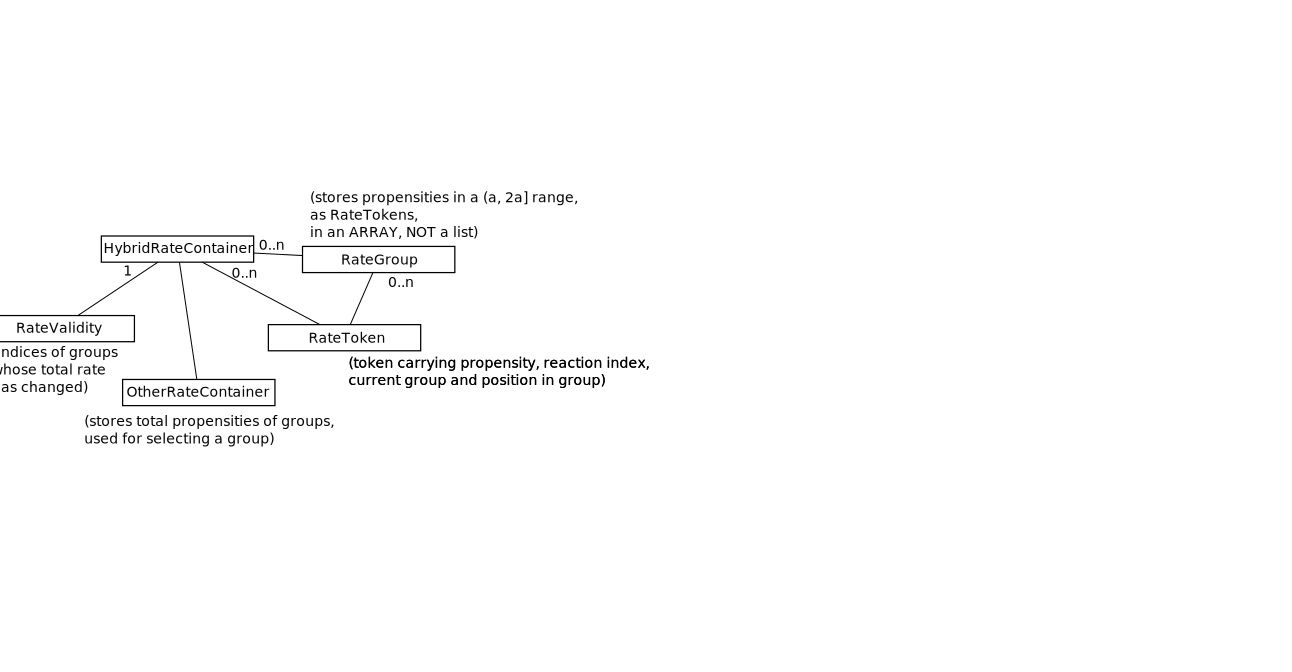
\includegraphics[width=0.9\textwidth]{hybrid_structure}
  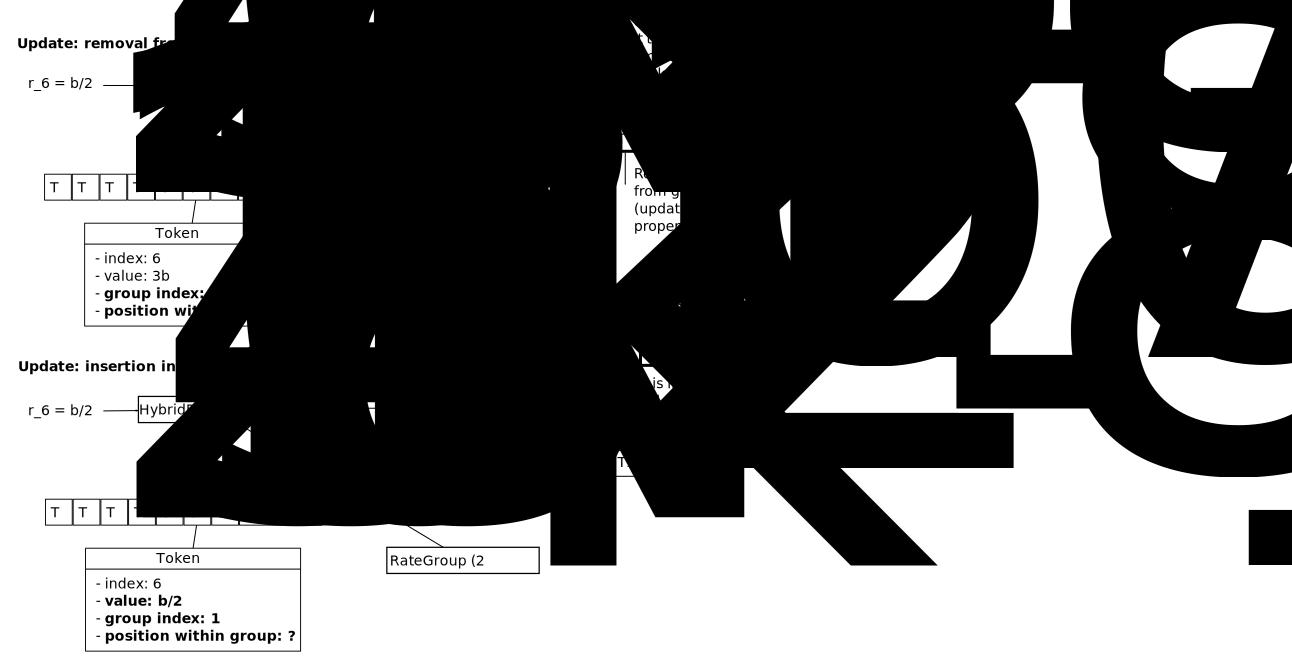
\includegraphics[width=0.9\textwidth]{hybrid_structure_update}
  \caption{Example of structure warranting optimal complexity. Propensities are stored in their \texttt{RateGroup} as \texttt{Token}s containing additional information, enabling $O(1)$ operations.}
  \label{fig:hybrid_structure}
\end {figure}

\reffigt{fig:hybrid_structure} shows an example of a design achieving optimal complexity using tokens to represent propensities. The costliest step is to determine the new group where to place the token. A logarithmic-like function has to be used, but if groups are delimited by powers of 2, more efficient low level functions can be used, such as \texttt{frexp} in C.

It is easy to design a similar structure without actual tokens, but in a language like C++, all these classes can be inlined and do not actually exist in the compiled code. If the design is careful enough, it can be both human-readable by using classes representing clear abstractions AND efficient.

\paragraph{Choice of base rate}

This is the trickiest part of the algorithm. The choice can be left to the user, but it is also possible to imagine a structure that adapts dynamically. We did not have time to put much thought into it, but some ideas would be
\begin{itemize}
  \item Create a base group at some arbirary rate. Each time a propensity (or too many propensities) falls into that group, subdivide the group into new groups, thus lowering the base group rate.
  \item Replace the base group with any container adapted to multinomial drawing, possible a hybrid drawing structure. If the value drawn falls into that group, the drawing method of the structure chosen is applied by reusing the same value to avoid additionnal random generator costs.
\end{itemize}

In both cases, the question is: at what point is it worth creating subgroups/substructures? This question has to be carefully analyzed before a choice of implementation is actually made.
